\chapter{Опорные поверхности}
\label{chap:surface-support}

\section{Определения}

Две гладкие поверхности $\Sigma_1$ и $\Sigma_2$ \index{касание!поверхности}\emph{касаются} в точке $p \z\in \Sigma_1 \cap \Sigma_2$, если у них в этой точке общая касательная плоскость.
В этом случае их нормали в $p$ либо равны, либо противонаправлены.
То есть, если поверхности ориентированы, то можно говорить о \index{сонаправленные и противонаправленные!поверхности}\emph{сонаправленном} или {}\emph{противонаправленном} касании в $p$.

Далее, если нашлась такая окрестность $U$ точки $p$, что $\Sigma_1\cap U$ лежит с одной стороны от $\Sigma_2$ в $U$, то говорят, что $\Sigma_2$ \index{локальная опорная}\emph{локально подпирает} $\Sigma_1$ в~$p$.
В этом случае поверхности обязаны касаться в $p$, выбрав их ориентации, можно считать, что они сонаправлены в $p$.

Допустим, что поверхности $\Sigma_1$ и $\Sigma_2$ касаются и сонаправлены в $p$.
Представим их локально графиками функций, скажем $f_1$ и $f_2$, в общих касательно-нормальных координатах при $p$.
Отметим, что $\Sigma_2$ локально подпирает $\Sigma_1$ в $p$ тогда и только тогда, когда неравенство
\[ f_1(x,y)\ge f_2(x,y)
\quad\text{или}\quad
f_1(x,y)\le f_2(x,y)\]
выполнено при всех $(x,y)$, достаточно близких к нулю.
В первом случае $\Sigma_2$ локально подпирает $\Sigma_1$ \index{опорная!поверхность}\emph{снаружи}, во втором --- \emph{изнутри}.



\begin{thm}{Предложение}\label{prop:surf-support}
Пусть $\Sigma_1$ и $\Sigma_2$ --- гладкие ориентированные поверхности.
Предположим, что $\Sigma_1$ локально подпирает $\Sigma_2$ изнутри в точке $p$ (эквивалентно, $\Sigma_2$ локально подпирает $\Sigma_1$ снаружи).
Тогда 
\[k_1(p)_{\Sigma_1}\ge k_1(p)_{\Sigma_2}\quad\text{и}\quad k_2(p)_{\Sigma_1}\z\ge k_2(p)_{\Sigma_2}.\]
\end{thm}

\begin{thm}{Упражнение}\label{ex:surf-support}
Постройте две поверхности $\Sigma_1$ и $\Sigma_2$ с общей точкой $p$ и общей нормалью при $p$, которые локально не подпирает друг друга в~$p$, но
$k_1(p)_{\Sigma_1}\z> k_1(p)_{\Sigma_2}$ и $k_2(p)_{\Sigma_1}\z> k_2(p)_{\Sigma_2}$.
\end{thm}

\parbf{Доказательство \ref{prop:surf-support}.}
Можно считать, что $\Sigma_1$ и $\Sigma_2$ --- графики $z\z=f_1(x,y)$ и $z=f_2(x,y)$ в общих касательно-нормальных координатах при $p$, так что $f_1\ge f_2$.

Пусть $\vec w\z\in \T_p\Sigma_1=\T_p\Sigma_2$ --- общий касательный единичный вектор.
Построим плоскость $\Pi$, через $p$, в направлении нормали $\Norm_p$ и ${\vec w}$.
Пусть $\gamma_1$ и $\gamma_2$ --- кривые пересечения $\Sigma_1$ и $\Sigma_2$ с $\Pi$.

Выберем ориентацию на $\Pi$, чтобы $\Norm_p$ указывал влево от ${\vec w}$.
Далее, параметризуем обе кривые в направлении ${\vec w}$ при $p$;
в этом случае они сонаправленны и $\gamma_1$ подпирает $\gamma_2$ справа в $p$.

\begin{wrapfigure}{o}{35 mm}
\vskip-6mm
\centering
\includegraphics{mppics/pic-80}
\vskip-0mm
\end{wrapfigure}

Из \ref{prop:supporting-circline}, получаем следующее неравенство на нормальные кривизны $\Sigma_1$ и $\Sigma_2$ в $p$ в направлении ${\vec w}$:
\[k_{\vec w}(p)_{\Sigma_1}\ge k_{\vec w}(p)_{\Sigma_2}.\eqlbl{kw>=kw}\]

\setlength{\columnseprule}{0.4pt}
\begin{multicols}{2}
Далее, из \ref{obs:k1-k2}, 
\[k_1(p)_{\Sigma_i}=\min_{\vec w}\set{k_{\vec w}(p)_{\Sigma_i}}{},\]
где $\vec w\in\T_p$ и $|\vec w|=1$.
Выберем ${\vec w}$ так, что 
\[k_1(p)_{\Sigma_1}\z=k_{\vec w}(p)_{\Sigma_1}.\]
Тогда из \ref{kw>=kw}, получим
\begin{align*}
k_1(p)_{\Sigma_1}&=k_{\vec w}(p)_{\Sigma_1}\ge
\\
&\ge k_{\vec w}(p)_{\Sigma_2}\ge
\\
&\ge\min_{\vec v}\set{k_{\vec v}(p)_{\Sigma_2}}{}=
\\
&=k_1(p)_{\Sigma_2}.
\end{align*}

\columnbreak

Аналогично, из \ref{obs:k1-k2},
\[k_2(p)_{\Sigma_i}=\max_{\vec w}\set{k_{\vec w}(p)_{\Sigma_i}}{},\]
где $\vec w\in\T_p$ и $|\vec w|=1$.
Выберем ${\vec w}$ так, что 
\[k_2(p)_{\Sigma_2}=k_{\vec w}(p)_{\Sigma_2},\]
и из \ref{kw>=kw},
\begin{align*}
k_2(p)_{\Sigma_2}&=k_{\vec w}(p)_{\Sigma_2}\le
\\
&\le k_{\vec w}(p)_{\Sigma_1}\le
\\
&\le\max_{\vec v}\set{k_{\vec v}(p)_{\Sigma_1}}{}=
\\
&=k_2(p)_{\Sigma_1}.
\end{align*}
\end{multicols}


В обоих случаях предполагается, что $\vec v\in\T_p$ и $|\vec v|=1$.\qeds



\begin{thm}{Следствие}\label{cor:surf-support}
Пусть $\Sigma_1$ и $\Sigma_2$ --- ориентированные гладкие поверхности.
Если $\Sigma_1$ локально подпирает $\Sigma_2$ изнутри в точке~$p$, то

\begin{subthm}{cor:surf-support:mean}
$H(p)_{\Sigma_1}\ge H(p)_{\Sigma_2}$;
\end{subthm}

\begin{subthm}{cor:surf-support:gauss}
Если $k_1(p)_{\Sigma_2}\ge 0$, то $K(p)_{\Sigma_1}\ge K(p)_{\Sigma_2}$.
\end{subthm}
 
\end{thm}



\parbf{Доказательство; \ref{SHORT.cor:surf-support:mean}.}
Следует из \ref{prop:surf-support}, поскольку $H=k_1+k_2$. 
%\[H(p)_{\Sigma_i}=k_1(p)_{\Sigma_i}+k_2(p)_{\Sigma_i}.\]



\parit{\ref{SHORT.cor:surf-support:gauss}.}
Поскольку $k_2(p)_{\Sigma_i}\ge k_1(p)_{\Sigma_i}$, и $k_1(p)_{\Sigma_2}\ge 0$, все главные кривизны 
$k_1(p)_{\Sigma_1}$, 
$k_1(p)_{\Sigma_2}$, 
$k_2(p)_{\Sigma_1}$ и 
$k_2(p)_{\Sigma_2}$ неотрицательны.
Из \ref{prop:surf-support}, получаем
\begin{align*}
K(p)_{\Sigma_1}&=k_1(p)_{\Sigma_1}\cdot k_2(p)_{\Sigma_1}\ge 
\\
&\ge k_1(p)_{\Sigma_2}\cdot k_2(p)_{\Sigma_2}=K(p)_{\Sigma_2}.
\end{align*}
\qedsf

\begin{thm}{Упражнение}\label{ex:positive-gauss-0}
Покажите, что на любой замкнутой поверхности в единичном шаре найдётся точка с гауссовой кривизной хотя бы~1.
Выведите отсюда, что любая замкнутая поверхность имеет точку с положительной гауссовой кривизной.
\end{thm}

{\sloppy

\begin{thm}{Упражнение}\label{ex:positive-gauss}
Покажите, что любая замкнутая поверхность, лежащая на расстоянии не более 1 от прямой, имеет точку с гауссовой кривизной не менее~1.
\end{thm}

}

\section{Выпуклые поверхности}

Поверхность называется \index{выпуклая!поверхность}\emph{выпуклой}, если она ограничивает выпуклую область.

\begin{thm}{Упражнение}\label{ex:convex-surf}
Покажите, что гауссова кривизна гладких выпуклых поверхностей неотрицательна.
\end{thm}

\begin{thm}{Продвинутое упражнение}\label{ex:convex-lagunov}
Пусть $R$ --- выпуклое тело в $\mathbb{R}^3$, ограниченное поверхностью с главными кривизнами, не превышающими~1.
Покажите, что $R$ содержит единичный шар.
\end{thm}

{\sloppy

Напомним, что область $R$ евклидова пространства называется {}\emph{строго выпуклой}, если для любых двух точек $x,y\in R$ любая точка $z$, лежащая между $x$ и $y$, находится во внутренности~$R$.

Любое открытое выпуклое множество строго выпукло. 
Куб, как и любой выпуклый многогранник, нестрого выпуклы.
Ясно, что \textit{замкнутая выпуклая область является строго выпуклой тогда и только тогда, когда её граница не содержит отрезков}.

}

\begin{thm}{Лемма}\label{lem:gauss+=>convexity}
Пусть $z=f(x,y)$ --- локальное представление гладкой поверхности $\Sigma$ в касательно-нормальных координатах при $p\in\Sigma$.
Если обе главные кривизны $\Sigma$ в~$p$ положительны,
то функция $f$ строго выпукла в окрестности нуля и имеет в нём локальный минимум.

В частности, касательная плоскость $\T_p$ локально подпирает $\Sigma$ снаружи в~$p$.
\end{thm}

\parbf{Доказательство.}
Поскольку обе главные кривизны положительны, \ref{cor:Shape(ij)} влечёт, что 
\[D^2_{\vec w}f(0,0)=\langle \Shape_p({\vec w}),{\vec w}\rangle\ge k_1(p)>0\] 
для любого единичного касательного вектора $\vec w\in\T_p\Sigma$ (в наших координатах $\vec w$ --- горизонтальный вектор).

Так как функция $(x,y,{\vec w})\mapsto D^2_{\vec w}f(x,y)$ непрерывна, $D^2_{\vec w}f(x,y)>0$, при любом $\vec w\ne 0$ и в любой точке $(x,y)$ в малой окрестности нуля.
Значит, $f$ строго выпукла в некоторой окрестности нуля (см. \ref{thm:Jensen}).

И наконец, у $f$ строгий локальный минимум в нуле,
ведь $\nabla f(0,0)\z=0$ и $f$ строго выпукла в окрестности нуля.
\qeds


\begin{thm}{Упражнение}\label{ex:section-of-convex}
Пусть $\Sigma$ --- гладкая поверхность (без границы) с положительной гауссовой кривизной.
Покажите, что любая компонента связности пересечения $\Sigma$ с плоскостью либо одна точка, либо гладкая кривая с ориентированной кривизной одного знака.
\end{thm}

\section{Признак выпуклости}

\begin{thm}{Теорема}\label{thm:convex-embedded}
Пусть $\Sigma$ --- открытая или замкнутая гладкая поверхность с положительной гауссовой кривизной.
Тогда $\Sigma$ ограничивает строго выпуклую область в $\mathbb{R}^3$.
\end{thm}

В доказательстве потребуется, что поверхность связна (это верно по определению);
иначе пара сфер дала бы контрпример.
Верно также, что \textit{любая замкнутая гладкая поверхность с неотрицательной гауссовой кривизной ограничивает выпуклую область},
но доказательство ощутимо сложней \cite{hadamard,gomes,sacksteder}.
Теорема остаётся верной для поверхностей с самопересечениями. 
Это доказано Джеймсом Стокером \cite{stoker}, который приписал результат Жаку Адамару, доказавшему близкое утверждение \cite[§ 23]{hadamard}.

Из доказательства ниже извлекается, что \textit{любая замкнутая связная локально выпуклая область евклидова пространства выпукла}.


\parbf{Доказательство.}
Поскольку гауссова кривизна положительна, можно считать, что главные кривизны положительны во всех точках.
Обозначим через $R$ область, ограниченную $\Sigma$, в которую указывает поле нормалей $\Norm$ на $\Sigma$.
(Область $R$ существует по \ref{clm:proper-divides}.)

Сначала покажем, что $R$ {}\emph{локально строго выпукла};
то есть для любой точки $p\in \Sigma$, пересечение $R$ и малого шара с центром в~$p$ строго выпукло.

Пусть $\Sigma$ локально задаётся графиком $z=f(x,y)$ в касательно-нормальных координатах при~$p$.
По \ref{lem:gauss+=>convexity}, функция $f$ строго выпукла в окрестности нуля.
В частности, пересечение малого шара с центром в $p$ и эпиграфа $z\ge f(x,y)$ строго выпукло.

Поскольку $\Sigma$ связна, связна и область $R$.
Более того, любые две точки внутри $R$ можно соединить ломаной во внутренности~$R$.



Допустим, что внутренность $R$ не выпукла;
то есть найдутся точки $x,y\in R$, и точка $z$ между $x$ и $y$, которая не лежит во внутренности~$R$.
Рассмотрим ломаную $\beta$ от $x$ до $y$ во внутренности~$R$.
Пусть $y_0$ --- первая такая точка на $\beta$, что хорда $[x,y_0]$ касается $\Sigma$, скажем в~$z_0$.

{

\begin{wrapfigure}{r}{43 mm}
\vskip-0mm
\centering
\includegraphics{mppics/pic-37}
\vskip-0mm
\end{wrapfigure}

Поскольку $R$ локально строго выпукла, $R\z\cap B(z_0,\epsilon)$ является строго выпуклой при достаточно малых $\epsilon>0$.
С другой стороны, $z_0$ лежит между двумя точками в пересечении $[x,y_0]\cap B(z_0,\epsilon)$.
Поскольку $[x,y_0]\subset R$, мы приходим к противоречию.

}

Следовательно, внутренность $R$ выпукла.
Отметим, что область $R$ есть замыкание своей внутренней части, поэтому $R$ также выпукла.

Поскольку $R$ является локально строго выпуклой, её граница $\Sigma$ не содержит отрезков прямых.
Следовательно, $R$  строго выпукла.
\qeds

\begin{thm}{Упражнение}\label{ex:surrounds-disc}
Предположим, что замкнутая поверхность $\Sigma$ ограничивает область, содержащую единичную окружность.
Покажите, что $K(p)\le 1$ для некоторой точки $p \in \Sigma$. 
\end{thm}

\begin{thm}{Упражнение}\label{ex:small-gauss}
Пусть $\Sigma$ --- замкнутая гладкая выпуклая поверхность диаметра не меньше $\pi$;
то есть существует пара точек $p,q\in\Sigma$ таких, что $|p-q|\ge \pi$.
Покажите, что $\Sigma$ имеет точку с гауссовой кривизной не более~1.
\end{thm}

\section{Ещё о выпуклости}

\begin{thm}{Теорема}\label{thm:convex-closed}
Любая замкнутая гладкая выпуклая поверхность $\Sigma$ является гладкой сферой;
то есть $\Sigma$ допускает гладкую регулярную параметризацию стандартной сферой $\mathbb{S}^2$.
\end{thm}

{

\begin{wrapfigure}[7]{r}{33 mm}
\vskip-8mm
\centering
\includegraphics{mppics/pic-78}
\end{wrapfigure}

\begin{thm}{Доказательство и упражнение}\label{ex:convex-proper-sphere}\\
Предположим, что выпуклая компактная область $R$ содержит начало координат в своей внутренности и ограничена гладкой поверхностью~$\Sigma$.

\begin{subthm}{ex:convex-proper-sphere:single}
Покажите, что любой луч, исходящий из начала координат, пересекает $\Sigma$ в единственной точке;
иначе говоря, существует такая положительная функция $\rho\:\mathbb{S}^2\z\to\mathbb{R}$, что $\Sigma$ состоит из точек $q\z=\rho(\xi)\cdot \xi$ для $\xi\in \mathbb{S}^2$.
\end{subthm}

\begin{subthm}{ex:convex-proper-sphere:smooth}
Покажите, что функция $\rho\:\mathbb{S}^2\to\mathbb{R}$ гладкая.
Выведите, что $\xi\z\mapsto \rho(\xi)\cdot \xi$ --- гладкая регулярная параметризация $\mathbb{S}^2\z\to \Sigma$.
\end{subthm}

\end{thm}

}



\begin{thm}{Теорема}\label{thm:convex-open}
Пусть $\Sigma$ --- открытая гладкая поверхность, ограничивающая строго выпуклую замкнутую область.
Тогда, в некоторой системе координат, $\Sigma$ задаётся графиком $z\z=f(x,y)$ выпуклой функции $f$, определённой на выпуклой открытой области $\Omega$ в $(x,y)$-плоскости.
Более того, $f(x_n,y_n)\to\infty$ если $(x_n,y_n)\to(x_\infty,y_\infty)\z\in \partial\Omega$.

\end{thm}

{

\begin{wrapfigure}{r}{28 mm}
\vskip-0mm
\centering
\includegraphics{mppics/pic-1181}
\vskip2mm
\end{wrapfigure}

\begin{thm}{Доказательство и упражнение}\label{ex:convex-proper-plane}
Предположим, что строго выпуклая замкнутая некомпактная область $R$ содержит начало координат во внутренней части и ограничена гладкой поверхностью~$\Sigma$.
Докажите следующее.

\begin{subthm}{ex:convex-proper-plane:a}
$R$ содержит луч, скажем $\ell$.
\end{subthm}

\begin{subthm}{ex:convex-proper-plane:b}
Любая прямая $m$, параллельная $\ell$, пересекает $\Sigma$ не более чем в одной точке.
\end{subthm}

\begin{subthm}{ex:convex-proper-plane:c}
В системе координат, с осью $z$ направленной по $\ell$, проекция $\Sigma$ на $(x,y)$-плоскость есть открытое выпуклое множество, скажем $\Omega$.
\end{subthm}

\begin{subthm}{ex:convex-proper-plane:d}
$\Sigma$ является графиком $z=f(x,y)$ гладкой выпуклой функции $f$, определённой на $\Omega$.
\end{subthm}

\begin{subthm}{ex:convex-proper-plane:e}
Докажите последнее утверждение в \ref{thm:convex-open}.
\end{subthm}

\end{thm}

}


\begin{thm}{Упражнение}\label{ex:open+convex=plane}
{\sloppy
Покажите, что любая открытая поверхность $\Sigma$ с положительной гауссовой кривизной является топологической плоскостью;
то есть существует вложение $\mathbb{R}^2\to\mathbb{R}^3$ с образом~$\Sigma$.

}

Попробуйте доказать, что $\Sigma$ является гладкой плоскостью;
то есть вложение $f$ можно сделать гладким и регулярным.
\end{thm}

{\sloppy

\begin{thm}{Упражнение}\label{ex:circular-cone}
Покажите, что любая открытая гладкая поверхность $\Sigma$ с положительной гауссовой кривизной
находится внутри бесконечного кругового конуса.
Другими словами, в некоторой системе координат, $\Sigma$ лежит в области $z \z\ge m \cdot\sqrt{x^2 + y^2}$ для положительной константы $m$.
\end{thm}

}

\begin{thm}{Упражнение}\label{ex:intK}
Предположим, что $\Sigma$ является гладкой выпуклой поверхностью положительной гауссовой кривизны
и $\Norm\:\Sigma\to \mathbb{S}^2$ --- её сферическое отображение.

\begin{multicols}{2}

\begin{subthm}{ex:intK:4pi}
Пусть $\Sigma$ замкнута.
Покажите, что $\Norm\:\Sigma\to \mathbb{S}^2$ является биекцией.
Выведите отсюда, что 
\[\iint_\Sigma K=4\cdot\pi.\]
\end{subthm}

\columnbreak

\begin{subthm}{ex:intK:2pi}
Пусть $\Sigma$ открыта.
Покажите, что $\Norm\:\Sigma\to \mathbb{S}^2$
задаёт биекцию на подмножество полусферы,
и выведите, что 
\[\iint_\Sigma K\le 2\cdot\pi.\]
\end{subthm}

\end{multicols}

\end{thm}

\chapter{Седловые поверхности}

\section{Определения}\label{sec:saddle}

\begin{wrapfigure}{r}{43 mm}
\vskip-16mm
\centering
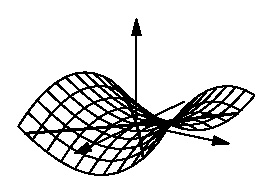
\includegraphics{asy/saddle}
\vskip0mm
\end{wrapfigure}

Поверхность называется \index{седловая поверхность}\emph{седловой}, если её гауссова кривизна в каждой точке неположительна;
другими словами, главные кривизны в каждой точке имеют противоположные знаки или хотя бы одна из них равна нулю.

Если гауссова кривизна отрицательна в каждой точке,
то поверхность называется {}\emph{строго седловой};
это означает, что главные кривизны имеют противоположные знаки в каждой точке.
В этом случае касательная плоскость не может подпирать поверхность даже локально --- при движении по поверхности в главных направлениях из точки, можно очутиться и выше и ниже её касательной плоскости.

\begin{thm}{Упражнение}\label{ex:convex-revolution}
Пусть $f\:\mathbb{R}\to\mathbb{R}$ --- гладкая положительная функция.
Покажите, что поверхность вращения графика $y\z=f(x)$ вокруг оси $x$
является седловой тогда и только тогда, когда $f$ выпукла; то есть если $f''(x)\ge0$ для любого~$x$.
\end{thm}

Поверхность $\Sigma$ называется \index{линейчатая поверхность}\emph{линейчатой}, если для каждой точки $p\in \Sigma$ существует прямая $\ell_p\subset \Sigma$, проходящий через $p$.

\begin{thm}{Упражнение}\label{ex:ruled=>saddle}
Покажите, что любая линейчатая поверхность седловая.
\end{thm}

\begin{thm}{Упражнение}\label{ex:saddle-convex}
Пусть $\Sigma$ --- открытая строго седловая поверхность, а $f\:\mathbb{R}^3\z\to\mathbb{R}$ --- гладкая выпуклая функция.
Покажите, что сужение $f$ на $\Sigma$ не имеет точки локального максимума.
\end{thm}


Направление на гладкой поверхности с нулевой нормальной кривизной называется \index{асимптотическое направление и линия}\emph{асимптотическим}.
Гладкая кривая, идущая всё время в асимптотическом направлении, называется
{}\emph{асимптотической линией}.\label{page:asymptotic line}

Напомним, что множество $R$ на плоскости называется \index{звёздное множество}\emph{звёздным}, если существует точка $p\in R$ такая, что для любой точки $x\in R$ отрезок $[p,x]$ принадлежит~$R$.

\begin{thm}{Продвинутое упражнение}\label{ex:panov}
Пусть $\gamma$ --- замкнутая гладкая асимптотическая линия
на графике $z\z=f(x,y)$ гладкой функции~$f$. 
Предположим, что график строго седловой в окрестности~$\gamma$.
Покажите, что область на $(x,y)$-плоскости, ограниченная проекцией $\bar \gamma$ кривой $\gamma$, не может оказаться звёздной. 
\end{thm}

\begin{thm}{Продвинутое упражнение}\label{ex:crosss}
Пусть $p$ --- точка на гладкой поверхности $\Sigma$ и $K(p)<0$.
Покажите, что существует окрестность $\Omega$ точки $p$ на $\Sigma$,
такая, что пересечение $\Omega$ с касательной плоскостью $\T_p$ представляет собой объединение двух гладких кривых, \index{трансверсальность}\emph{трансверсально пересекающихся} в точке~$p$;
то есть их векторы скорости линейно независимы в $p$.
\end{thm}



\section{Критерий горбушек}

Обратите внимание, что \textit{замкнутая поверхность не может быть седловой}.
Действительно, пусть $\Sigma$ --- замкнутая поверхность.
Рассмотрим наименьшую сферу, которая окружает~$\Sigma$.
Эта сфера обязана подпирать $\Sigma$ в некоторой точке.
Согласно \ref{prop:surf-support}, в этой точке у $\Sigma$ главные кривизны одного знака.
Следующее более общее утверждение использует похожую идею.

\begin{thm}{Лемма}\label{lem:convex-saddle}
Пусть $\Sigma$ --- компактная седловая поверхность, и её граничная линия лежит в замкнутой выпуклой области~$R$.
Тогда вся поверхность $\Sigma$ лежит в~$R$.
\end{thm}

{

\begin{wrapfigure}{r}{46 mm}
\vskip-8mm
\centering
\includegraphics{mppics/pic-73}
\vskip-4mm
\end{wrapfigure}

\parit{Замечание.}
Для строго седловых поверхностей, лемму можно вывести из \ref{ex:saddle-convex}.

\parbf{Доказательство.}
Допустим, что существует точка $p\in \Sigma$,  не лежащая в~$R$.
Тогда найдётся плоскость $\Pi$, отделяющая $p$ от $R$, см.~\ref{lem:separation}.
Обозначим через $\Sigma'$ ту часть $\Sigma$, которая лежит с $p$ на одной стороне~$\Pi$.

}

Так как $\Sigma$ компактна, её можно окружить сферой;
пусть $\sigma$ --- окружность пересечения этой сферы с $\Pi$.
Рассмотрим наименьший сферический купол $\Sigma_0$ с границей $\sigma$, который окружает~$\Sigma'$.

$\Sigma_0$ подпирает $\Sigma$ в некоторой точке~$q$.
Не умаляя общности, можно предположить, что $\Sigma_0$ и $\Sigma$ сонаправлены в $q$, и у $\Sigma_0$ положительные главные кривизны.
В этом случае, $\Sigma_0$ подпирает $\Sigma$ снаружи,
и из \ref{cor:surf-support}, $K(q)_\Sigma\z\ge K(q)_{\Sigma_0}>0$ --- противоречие.
\qeds


\begin{thm}{Упражнение}\label{ex:proper-saddle}
{\sloppy 
Постройте собственную седловую поверхность, которая не лежит в выпуклой оболочке своей граничной линии.
(Согласно \ref{lem:convex-saddle}, она некомпактна.)

}
\end{thm}

\begin{thm}{Упражнение}\label{ex:length-of-bry}
Предположим, что точка $p$ лежит на компактной гладкой седловой поверхности $\Delta$ с границей на единичной сфере с центром в~$p$.
Докажите, что если $\Delta$ является топологическим диском, то $\length(\partial\Delta)\ge 2\cdot\pi$.

Покажите, что это перестаёт быть верным без предположения, что $\Delta$ топологический диск.
\end{thm}

\parit{Замечание.}
На самом деле $\area \Delta\ge \pi$;
то есть единичный круг имеет минимальную возможную площадь среди поверхностей из упражнения.
Это выводится из так называемой \index{формула коплощади}\emph{формулы коплощади}.

\begin{thm}{Упражнение}\label{ex:circular-cone-saddle}
Покажите, что открытая седловая поверхность
не может лежать внутри бесконечного кругового конуса. 
\end{thm}

Топологический диск $\Delta$ на поверхности $\Sigma$ называется \index{горбушка}\emph{горбушкой} поверхности $\Sigma$, если его граничная линия $\partial\Delta$ лежит в некоторой плоскости $\Pi$, а $\Delta \setminus \partial \Delta$ лежит строго с одной стороны от $\Pi$.

\begin{thm}{Предложение}\label{prop:hat}
Гладкая поверхность $\Sigma$ является седловой тогда и только тогда, когда на ней нет горбушек.
\end{thm}

Седловая поверхность может содержать замкнутую плоскую кривую.
Например, гиперболоид $x^2+y^2-z^2=1$ пересекается по единичной окружности с плоскостью $(x,y)$.
Однако, согласно предложению (и лемме), на седловой поверхности, плоская кривая не может ограничивать топологический диск (как и любое компактное множество).


\parbf{Доказательство.}
Так как плоскость выпукла, необходимость следует из \ref{lem:convex-saddle};
остаётся доказать достаточность.

Допустим, что $\Sigma$ не седловая; то есть у неё есть точка $p$ со строго положительной гауссовой кривизной;
иначе говоря, её главные кривизны $k_1(p)$ и $k_2(p)$ одного знака.
Давайте считать, что $0 < k_1(p) \z\le k_2(p)$, другой случай аналогичен.

Пусть $z=f(x,y)$ --- локальное представление $\Sigma$ в касательно-нормальных координатах при~$p$.
Рассмотрим множество $F_\epsilon$ в плоскости $(x,y)$, определяемое неравенством $f(x,y)\le \epsilon$.
Согласно \ref{lem:gauss+=>convexity}, функция $f$ выпукла в малой окрестности $(0,0)$.
Следовательно, $F_\epsilon$ выпукло при достаточно малых $\epsilon>0$.
В частности, $F_\epsilon$ --- топологический диск.

Отображение $(x,y)\mapsto (x,y,f(x,y))$ есть гомеоморфизм из $F_\epsilon$
в
\[\Delta_\epsilon=\set{(x,y,f(x,y))\in \mathbb{R}^3}{f(x,y)\le \epsilon};\]
следовательно,
$\Delta_\epsilon$ --- топологический диск при любом достаточно малом $\epsilon>0$.
Граничная линия $\Delta_\epsilon$ лежит в плоскости $z=\epsilon$, и весь диск лежит ниже неё;
то есть $\Delta_\epsilon$ является горбушкой~$\Sigma$.
\qeds

Следующее упражнение показывает, что на самом $\Delta_\epsilon$ деле гладкий диск.
Из него выводится более сильный вариант критерия горбушек (\ref{prop:hat});
а именно, в определении горбушек можно предполагать, что диск является гладким.

\begin{thm}{Упражнение}\label{ex:disc-hat}
Пусть $f\:\mathbb{R}^2\to\mathbb{R}$ --- гладкая строго выпуклая функция с минимумом в нуле.
Покажите, что для любого $\epsilon>0$, множество $F_\epsilon$ в графике $z=f(x,y)$, определяемое неравенством $f(x,y)\le \epsilon$, есть гладкий диск;
то есть существует диффеоморфизм из
$F_\epsilon$ на единичный диск $\Delta\z=\set{(x,y)\in\mathbb{R}^2}{x^2+y^2\le 1}$.
\end{thm}

\begin{thm}{Упражнение}\label{ex:saddle-linear}
Пусть $L\:\mathbb{R}^3\to\mathbb{R}^3$ --- \index{аффиннoe преобразование}\emph{аффиннoe преобразование}; то есть биекция $\mathbb{R}^3\to\mathbb{R}^3$, переводящая любую плоскость в плоскость. 
Покажите, что для любой седловой поверхности $\Sigma$ образ $L(\Sigma)$ также седловая поверхность.
\end{thm}


%???Monkey saddle


\section{Седловые графики}

Следующая теорема доказана Сергеем Бернштейном \cite{bernstein}.
\index{теорема Бернштейна}

\begin{thm}{Теорема}\label{thm:bernshtein}
Если гладкая функция $f\:\mathbb{R}^2\to\mathbb{R}$ имеет строго седловой график $z=f(x,y)$, то она неограничена;
то есть нету константы $C$, при которой неравенство 
$|f(x,y)|\le C$ выполнялось бы при любых $(x,y)\in\mathbb{R}^2$.
\end{thm}

По теореме, седловой график не может лежать между двумя горизонтальными плоскостями.
Вместе с \ref{ex:saddle-linear} это влечёт, что седловые графики не могут находиться между двумя параллельными плоскостями.
Следующее упражнение показывает, что теорема не применима к седловым поверхностям, не являющимся графиками.

\begin{thm}{Упражнение}\label{ex:between-parallels}
Постройте открытую строго седловую поверхность, лежащую между двумя параллельными плоскостями.
\end{thm}


Бывают функции со строго седловым графиком, ограниченные лишь с одной стороны.
Поскольку $\exp(x-y^2)>0$, следующее упражнение даёт такой пример.
То есть в доказательстве теоремы нам придётся использовать и верхнюю и нижнюю оценку на $f$.

\begin{thm}{Упражнение}\label{ex:one-side-bernshtein}
Покажите, что график
$z=\exp(x-y^2)$
является строго седловым.
\end{thm}

Следующее упражнение даёт усиление теоремы Бернштейна.

\begin{thm}{Продвинутое упражнение}\label{ex:saddle-graph}
Пусть $\Sigma$ --- открытая гладкая строго седловая поверхность в $\mathbb{R}^3$.
Предположим, что существует такое компактное подмножество $K\subset \Sigma$, что дополнение $\Sigma\setminus K$ является графиком $z=f(x,y)$ гладкой функции, определённой в открытой области плоскости $(x,y)$.
Покажите, что вся поверхность $\Sigma$ является графиком.
\end{thm}


Следующая лемма похожа на \ref{ex:length-of-bry};
она потребуется в доказательстве теоремы \ref{thm:bernshtein}.

\begin{thm}{Лемма}\label{lem:region}
Не существует собственной строго седловой гладкой поверхности, с граничной линией в плоскости $\Pi$ и, расположенной на ограниченном расстоянии от некоторой прямой в $\Pi$.
\end{thm}

\parbf{Доказательство.}
Воспользовавшись \ref{ex:saddle-linear}, лемму можно переформулировать следующим образом:
\textit{не существует собственной строго седловой гладкой поверхности 
с граничной линией в $(x,y)$-плоскости,
содержащейся в бесконечном параллелепипеде следующего вида:}
\[R=\set{(x,y,z)\in\mathbb{R}^3}{0\le z\le r,\  0\le y\le r}.\]

Предположим обратное, пусть $\Sigma$ --- такая поверхность.
Рассмотрим проекцию $\hat \Sigma$ на $(x,z)$-плоскость.
Она лежит в верхней полуплоскости, но ниже линии $z=r$.

Рассмотрим открытую верхнюю полуплоскость
\[H=\set{(x,z)\in \mathbb{R}^2}{z> 0}.\] 
Пусть $\Theta$ --- компонента связности дополнения $H\setminus \hat \Sigma$, содержащая точки выше линии $z=r$.

Заметим, что $\Theta$ выпукла.
Если это не так, то найдётся отрезок $[p,q]$ с $p,q\in \Theta$, отсекающий от $\hat\Sigma$ компактный кусок.
\begin{figure}[!ht]
\vskip-1mm
\centering
\includegraphics{mppics/pic-74}
\vskip-1mm
\end{figure}
Пусть $\Pi$ --- плоскость через $[p,q]$, перпендикулярная $(x,z)$-плоскости, она отсекает от $\Sigma$ компактную область $\Delta$.
Применив \ref{lem:reg-section}, можно считать, что $\Delta$ --- компактная поверхность с краем в $\Pi$, и остальная часть $\Delta$ лежит строго с одной стороны от $\Pi$.
Так как плоскость $\Pi$ выпукла, приходим к противоречию с \ref{lem:convex-saddle}.

Итак, $\Theta$ является открытым выпуклым множеством $H$, которое содержит все точки выше $z=r$.
По выпуклости, вместе с любой точкой $w$ множество $\Theta$ содержит все точки на лучах, которые начинаются в $w$ и \textit{направлены вверх}; то есть в направлениях с положительной $z$-координатой. 
Другими словами, вместе с любой точкой $w$
множество $\Theta$ содержит все точки с большей координатой $z$.
\begin{figure}[!ht]
\vskip-1mm
\centering
\includegraphics{mppics/pic-75}
\vskip-1mm
\end{figure}
Так как $\Theta$ открыто, оно описывается неравенством $z>r_0$.
Отсюда вытекает, что плоскость $z=r_0$ подпирает $\Sigma$ в некоторой точке (на самом деле во многих точках).
Применив \ref{prop:surf-support}, приходим к противоречию.
\qeds


%Note that the same proof goes through if one replaces the condition $0 \leq y \leq r$ in \ref{eq:R-bernstein} with $0 \leq y \leq h(x)$ for some positive continuous function $h$.

\parbf{Доказательство \ref{thm:bernshtein}.}
Пусть $\Sigma$ --- график $z=f(x,y)$.
Предположим обратное, а именно, что $\Sigma$ лежит между двумя плоскостями $z=\pm C$. 

Функция $f$ не может быть постоянной.
Следовательно, касательная плоскость $\T_p$ в некоторой точке $p\in\Sigma$ не горизонтальна.

Обозначим через $\Sigma^+$ часть $\Sigma$, лежащую выше $\T_p$.
В ней есть как минимум две связные компоненты, которые приближаются к $p$ с обеих сторон 
вдоль главного направления с положительной главной кривизной.
Иначе нашлась бы кривая в $\Sigma^+$, подходящая к $p$ с обеих сторон.
Она бы отсекла от $\Sigma$ топологический диск, скажем $\Delta$, с граничной линией не ниже $\T_p$ и некоторыми точками строго ниже $\T_p$,
а это противоречит \ref{lem:convex-saddle}. 
Итак, в $\Sigma^+$ две связные компоненты или больше.

\begin{figure}[!ht]
\vskip-1mm
\centering
\includegraphics{mppics/pic-76}
\caption*{Поверхность $\Sigma$, вид сверху.}
\vskip0mm
\end{figure}

Пусть $\T_p$ задаётся уравнением $z=h(x,y)=a\cdot x+b\cdot y+c$.
Тогда $\Sigma^{+} = \set{(x,y,f(x,y))\in \Sigma}{h(x,y) \leq f(x,y)}$.
Следовательно, $\Sigma^{+}$ содержит связное множество
\[R_-=\set{(x,y,f(x,y))\in\Sigma}{h(x,y)< -C}\] 
и не пересекается с  
\[R_+=\set{(x,y,f(x,y))\in\Sigma}{h(x,y)> C} . \]
Значит одна из связных компонент, скажем, $\Sigma^+_0$, лежит в полосе
\[R_0=\set{(x,y,f(x,y))\in\Sigma}{|h(x,y)|\le  C}.\]
Это множество находится на ограниченном расстоянии от прямой пересечения $\T_p$ с $(x,y)$-плоскостью.

Подвинем $\T_p$ чуть вверх и отсечём от $\Sigma^+_0$ часть выше полученной плоскости, назовём её $\bar\Sigma^+_0$.
Применив \ref{lem:reg-section},
можно считать, что $\bar\Sigma^+_0$ --- гладкая поверхность с границей;
по построению, её граничная линия лежит в плоскости.
Расстояние от полученной поверхности $\bar\Sigma^+_0$ до прямой всё ещё ограничено,
что невозможно по \ref{lem:region}.
\qeds


\section{Замечания}

Для нестрого седловых поверхностей, теорема Бернштейна и лемма в её доказательстве не верны;
контрпримеры можно найти среди цилинтрических поверхностей, см. конец \ref{sec:shape}.
На самом деле других примеров нет;
доказательство основано на той же идее, но сложней.

Согласно критерию горбушек \ref{prop:hat}, седловые поверхности можно определять как гладкие поверхности без горбушек.
Это определение работает для произвольных поверхностей, не обязательно гладких.
Многие из приведённых результатов, например, характеристика седловых графиков Бернштейна, остаются верными для таких обобщённых седловых поверхностей.
Однако этот класс поверхностей пока что недостаточно изучен; см. \cite[глава 4]{alexander-kapovitch-petrunin2019} и ссылки там.

